\title{Part-of-Speech Tagging Using Hidden Markov Models}
\author{
  Alankar Kotwal\\
  \texttt{12D070010}
  \and
  Sharad Mirani\\
  \texttt{12D070003}
  \\
}
\date{Department of Electrical Engineering, IIT Bombay}

\documentclass[11pt]{article}

\usepackage{amsmath,cancel}
\usepackage{amssymb}
\usepackage{hyperref}
\usepackage{ulem,color}
\usepackage[margin=0.75in]{geometry}
\usepackage{cite}
\usepackage{lettrine}
\usepackage{graphicx}
\usepackage{float}
\usepackage{subcaption}
\usepackage{enumitem}
\usepackage{hyperref}

%\pagenumbering{gobble}

\begin{document}
\maketitle

\begin{abstract}
\lettrine[lines=2]{T}{he} aim of the field of Natural Language Processing is to enable text-based communication between humans and computers. In particular, many challenges in the field focus on language understanding that is, enabling computers to derive meaning from human or natural language input, and others involve natural language generation. A basic component of language understanding is extracting the role of words used in the context of a sentence. We reason why parts of speech are a good way to qualify the roles of words in a sentence. We then motivate why Hidden Markov Models (HMMs) are a good solution to this problem. Finally, we show an implementation of part-of-speech tagging with HMMs and present results of using the model on real-life sentences. Reasons for failure and areas of improvement are pointed out.
\end{abstract}

\section{Introduction}
The field of Natural Language Processing (NLP)~\cite{wiki:nlp} strives to get computers to understand natural human language and generate appropriate responses to it. NLP aims to solve a number of problems, prominent among these being Automatic Summarization, Machine Translation, Morphological Segmentation and so on. Part-of-speech (POS) tagging~\cite{wiki:pos} is an important pre-processing step in many of these tasks. A good example~\cite{so:uses} goes as follows. Consider automatic translation applied to the sentence
%
$$\text{I fish a fish.}$$
%
Without tagging, `fish' would be translated the same way in both cases, which would lead to a wrong transduction. However, after POS tagging, the sentence would be
%
$$\text{I/PRP fish/VBP a/DT fish/NN ./.}$$
%
From a computer's point of view, both words are now distinct. The computer now has a way of distinguishing the word `fish' as used in both contexts.

The roles of words in a sentence and their classification into parts of speech are intimately connected. For example, consider the sentence
%
$$\text{She was very understanding.}$$
%
The piece of information that `she' is what the sentence talks about and that `understanding' is a quality of `she' is very important in understanding the sentence. The subject, `she', is classified as the noun and the quality, `understanding', is classified as an adjective. This is how this classification helps us understand natural language. Thus, POS tagging is an important and relevant problem in modern computatinal linguistics.

\section{Justifying Non-triviality}
One might question the non-triviality of such a task. For instance, one might argue that POS tagging can easily be achieved by maintaining a list of words and their corresponding part of speech. Indeed, the first part-of-speech taggers were rule-based. This, however, is doomed to failure; consider the use of `understanding' in the two sentences below:
%
$$\text{She was very understanding. \quad \quad Are you understanding this?}$$
%
A rule-based tagger would assign the same part of speech to `understanding' in both sentences. However, we clearly see that `understanding' in the first sentence, being a quality of `she', is an adjective while `understanding' in the second sentence is used as a present participle.

However, given the `context' of the sentence, it is possible to disambiguate the part of speech. In the case of the above sentences, we need only look at the sentence before `understanding' to discern the part of speech for it. This turns to be true in general because context in a language lies in the sequence of words used in a sentence.

\section{The Hidden Markov Model}
The above example, in fact, motivates why Hidden Markov Models are such a good fit for this problem. Given the tags for words before a particular word, it is possible to disambiguate the tag for this particular word. We assume, here, that the immediately previous word is sufficient for this; a more advanced approach would take into account more previous words.

Our states, then, are the tags associated with the words in a sentence. The transitions for the Hidden Markov Model can then be represented as a Markov chain which, in a toy model, would look like Fig~\ref{fig:hmm-trans}. Each state of the Markov chain emits words as seen in Fig~\ref{fig:hmm-emis}.

\begin{figure}[!t]
\begin{subfigure}[t]{0.5\textwidth}
	\centering
	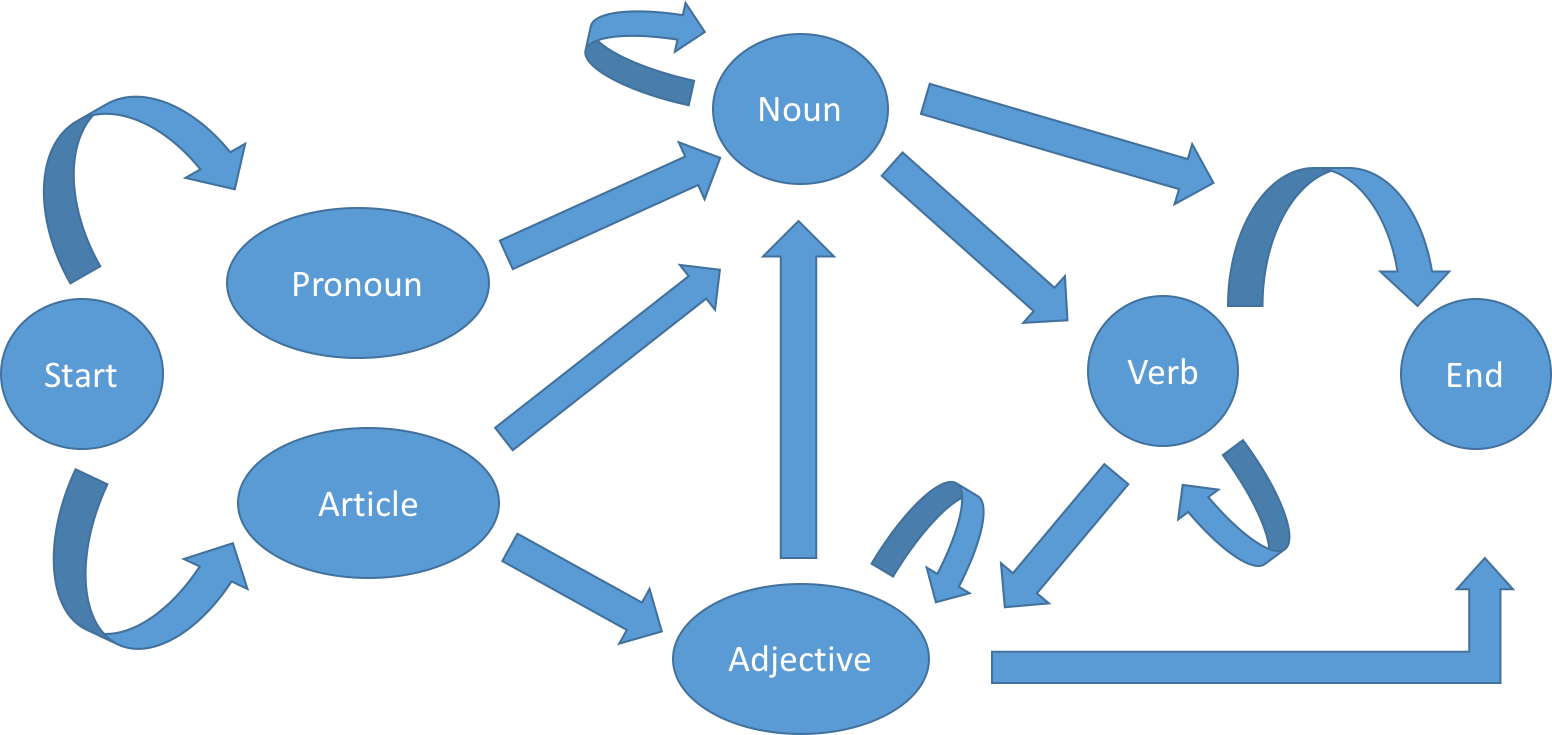
\includegraphics[height=1.6in]{hmm-trans}
	\caption{The Markov Chain for the state transitions in the HMM model}
	\label{fig:hmm-trans}
\end{subfigure}~
\begin{subfigure}[t]{0.5\textwidth}
	\centering
	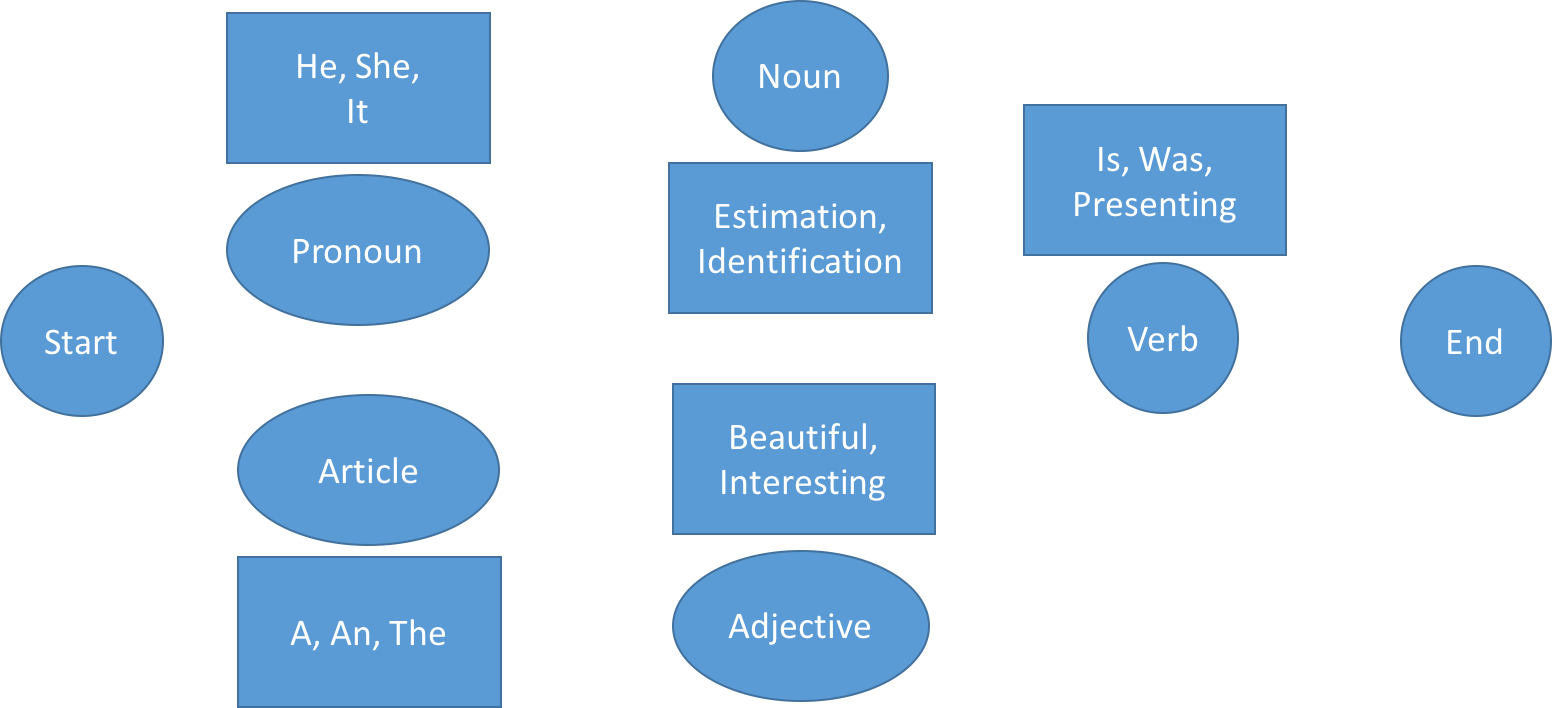
\includegraphics[height=1.6in]{hmm-emis}
	\caption{Emissions in the HMM model}
	\label{fig:hmm-emis}
\end{subfigure}
\caption{Hidden Markov Model construction}
\label{fig:hmm}
\end{figure}

It is clear, then, that the `context' is captured in the transition probabilities and the empirical knowledge that certain words are most often used as a particular part of speech is encoded in the emission probabilities. Given this construction of the HMM, it is now straightforward to train it given a tagged training dataset and use it for tagging sentences. 

\section{Implementation}

\subsection{Our Dataset}
We choose the datasets from~\cite{dataset} after getting rid of the chunking labels in it. These are sentences from the Wall Street Journal. The dataset has sentences of the form
%
$$\text{Confidence/NN in/IN the/DT pound/NN is/VBZ expected/VBN to/TO take/VB a/DT sharp/JJ dive/NN}$$
%
Each sentence has words tagged with their part of speech. We use this data to derieve the transition and emission probabilities as outlined below. The tags are explained in~\cite{tags}.

\subsection{Training}
Computers cannot, of course, understand sentences and words. Storage and search in raw form is tedious because sentences can be of variable length and search requires exact matching with the entire wordbase (which, as we will see, can easily run into several thousands). We therefore decide on a HashMap representation. Words are converted to all lowercase letters and stored in a HashMap, yielding a unique identifier for each word. An analogous thing is done for POS tags.

Given this representation, we commence training of the Hidden Markov Model. We parse the sentence and the tags, adding a new entry into the HashMaps for words or symbols when a new word or symbol is encountered. At every stage, we increment the transition matrix entry for the transition from the previous tag to the present by one, and increment the number of emissions of the current word from the current tag by one. At the end of training, we normalize the matrices so that the rows of both matrices represent distributions over next state and current emission respectively. It is a common practise to add a small constant to the transition matrix in case a transition is unseen in real data, but is necessitated by the fact that with very high probability, the incumbent word can be emitted only by a certain part of speech.

Handling unknown words is accomplished by creating a new dummy word $\_\_ UNK \_\_$. We set emission probabilities such that each state has equal probability of emitting this word, and hence unknown words are tagged purely on context.

\subsection{Testing}
Testing, then, with the transition and emission martices, is trivial. We parse and hash the input sequence and run the sequence of identification numbers for words through the Viterbi decoder to get a maximum-likelihood estimate of the underlying POS sequence.

\section{Results}
We present some significant results below:
\begin{enumerate}
\item A set is a collection. $\rightarrow$ \{DT, NN, VBZ, DT, NN, .\}
\item Did you set my alarm? $\rightarrow$ \{VBD, PRP, VB, PRP\$, NN, .\}
\end{enumerate}
%
This pair of examples is particularly interesting because the word `set' is used in different contexts here. Notice how the model is able to capture the difference and classify it correctly as a noun in the first sentence and as a verb in the second.
%
\begin{enumerate}[resume]
\item When bank financing for the buy-out collapsed last week, so did UAL's stock. $\rightarrow$ \{WRB, NN, NN, IN, DT, NN, VBD, JJ, NN, ,, RB, VBD, NNP, POS, NN, .\}
\end{enumerate}
%
This shows how the output stays correct even in long sentences and with the use of possessives like ``UAL's"
%
\begin{enumerate}[resume]
\item This is my awesome project for Estimation. $\rightarrow$ \{DT, VBZ, PRP\$, JJ, NN, IN, NN, .\}
\end{enumerate}
%
This last example is particularly fascinating because the words `awesome' and `Estimation' were not present in the dataset. Hence, the Markov model had no help from emission probabilities. The POS, in this case, were figured out completely on the basis of the context. This illustrates the power of the model to guess POS even in the presence of unknown words.

Our training dataset had 8637 sentences, spanning 45 POS and 17260 words. We tested the model on a dataset of 1952 sentences, with a remarkable error rate of $5.17\%$.

\section{Where do we fail?}
To improve upon any work, we must list failure cases. Here are ours:
\begin{enumerate}
\item Unknown words are a huge source of errors. For instance, change the last result above to ``This is my course project for Estimation.", and the tag does not change if `course' was not in the dataset. There is not much we can do in this case without the meaning of `course'.
\item Confusing usage: How does one tell if `set' is present or past in a sentence like ``You set my alarm."? This can be gleaned only from the global context and tone of the sentence's environment.
\item The assumption that the immediately previous word is sufficient might not hold. People try extending the HMM to two immediately previous words in order to resolve this. This approach is called a Trigram Hidden Markov model.
\end{enumerate}

\section{Conclusion}
We theoretically understood the reason HMMs are a good way of doing POS tagging. Then, we successfully trained and tested a POS tagger on a considerable sized dataset and have demonstrated its abilities to discern context as well as classify POS accurately. This has turned out to be a good exercise on the boundary of statistics and linguistics.
%Our implementation and trained POS tagger can be found \href{https://github.com/alankarkotwal/pos-tagging}{here}.

\section{Acknowledgements}
The authors would like to thank the course instructor for having given them the opportunity to explore applications of estimation theory in their fields of interest. They acknowledge the role of the cited resources in achieving an understanding of the subject matter and implementing it.

\bibliographystyle{unsrt}
\bibliography{report}

\end{document}